\documentclass[twocolumn]{article}
\setlength{\columnsep}{30pt}
\usepackage{a4wide,url,changebar}
\usepackage{fancyhdr,xspace}
\usepackage[pdftex]{graphicx}
\usepackage{amsfonts}
\usepackage{amsmath}
\usepackage{amssymb}
\usepackage{fix-cm}
\usepackage{euler}
\usepackage{amssymb}
\usepackage{eso-pic}
\usepackage{helvet}
\usepackage{url}
\pagestyle{fancy}


\newcommand{\inlinegraphic}[2]{
  \dimendef\grafheight=255\dimendef\grafvshift=254
  \grafheight=#1
  \grafvshift=-0.5\grafheight
  \advance\grafvshift by 0.5ex
  \raisebox{\grafvshift}{\includegraphics[height=\grafheight]{#2}\xspace}
}

\fancyhead[L]{\url{theorymine.co.uk}}
\fancyhead[R]{\inlinegraphic{1cm}{images/smalllogo_new.png}}
\fancyfoot[C]{\rm\thepage}


\title{About Your Theorem}
\author{TheoryMine}
\date{\today}


\newcommand{\nat}{\mathbb{N}}
\newcommand{\bool}{\text{Bool}}
\newcommand{\nl}{\\}

\begin{document}
\maketitle

\section{Recursion and Induction}
\label{recursion}



\begin{figure}[hbt]
% \topline
\begin{center}
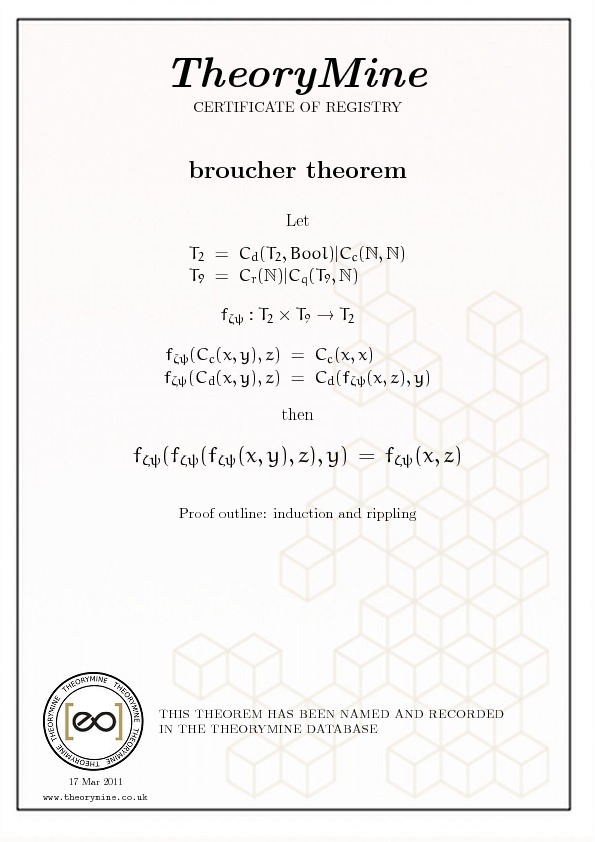
\includegraphics[width=6cm]{certificate_image.jpg}
\end{center}
\caption{Your certificate}
\label{certificate}
% \botline
\end{figure}

Your certificate is given in Figure \ref{certificate}.  In order to understand
it, it is first necessary to understand the concepts of {\em recursion} and {\em
  induction}.  In this section we provide an elementary introduction to these
concepts for those not already familiar with them.  Those who do not need this
introduction can proceed to \S\ref{objects}.

Both new mathematical objects (see \S\ref{objects}) and new defined functions
(see \S\ref{functions}) are defined using recursion. This is a form of
definition in which the body of the definition contains the thing being
defined. This sounds circular, but it need not be. Similarly, theorems about
recursive objects and functions are usually proved by mathematical induction. At
first sight, this form of proof can also appear to be circular, but it is not
once you understand it.

\subsection{The Natural Numbers}
\label{naturals}

Consider, the following recursive definition of the, so called, {\em natural
  numbers}, i.e., the non-negative whole numbers $0, 1, 2, 3, \ldots$.
\begin{eqnarray}
 \nat & = & 0 |
Suc(\nat) \label{nats}
\end{eqnarray}
where $Suc$ is called the $successor$ $function$. This definition is in Backus-Naur
Form\footnote{\url{http://en.wikipedia.org/wiki/Backus_Naur_Form}} ({\sc
  bnf}). $\nat$, the set of natural numbers, which is being defined, is to the left
of the $=$ sign. On the right of the $=$ sign is the body of the
definition. This consists of two cases, separated by a vertical line $|$. Any
particular natural number corresponds to one of these cases.  Note that $\nat$
occurs in the second case $Suc(\nat)$. This is a {\em step case}. The other case,
$0$, is a {\em base case}. 

The occurrence of a concept in the body of its own definition is an indication
that the definition is {\em recursive}. Think of this recursive definition, not
as a circle, but as a spiral.  $0$ is at the centre of the spiral; each
application of $Suc$ winds the spiral out by a complete circuit.  This process
generates a representation of the natural numbers of the form $0, Suc(0), Suc(Suc(0)),
Suc(Suc(Suc(0))), \ldots$, where each application of $Suc$ increases the number by
1. This representation is due to the mathematician Giuseppe
Peano\footnote{\url{http://en.wikipedia.org/wiki/Peano_axioms}} (1858-1932).

$0$ and $Suc$ are called {\em constructor functions}, because they are used to
construct new types of mathematical objects. Note that constructor functions are
{\em deliberately} not defined. They are taken as primitive mathematical objects
and are used in the definitions of other mathematical objects and defined
functions. Definitions have to stop unfolding at some point, and that point is
with the constructor functions.

The boolean truth values, $true$ and $false$, can be
defined by a degenerate form of recursion, in which there are two base
cases and no step cases: $Bool = true | false$. 

We will use $Bool$ and $\nat$ as the basis for defining new sets of recursively
defined mathematical objects, such as those explained in \S\ref{objects}
below. They will occur as some of the inputs to constructor functions.

\subsection{The Addition Function}
\label{addition}

The function $+$ can also be defined recursively. It takes
two members of $\nat$ as inputs and returns one as output.  It
also has a base case and a step case.

\begin{eqnarray}
 + & : & \nat \times \nat \rightarrow \nat \label{type} \\
0+y & = & y  \label{base} \\
Suc(x)+y & = & Suc(x+y) \label{step}
\end{eqnarray}

Line (\ref{type}) says that + takes two natural numbers as inputs and
outputs one natural number. Lines (\ref{base}) and (\ref{step}) constitute the
recursive definition of +. The formulae to the left of the = sign are the {\em heads}
of the definition and those to the right are the {\em body}.  Line (\ref{base})
is a base case, in which + does not occur on the right hand side. Line
(\ref{step}) is a step case, in which + {\em does} occur on the right hand side.
The recursion is on $x$, the first input of +.  $x$ is called the {\em recursion
  variable}.  Note that for each of the two cases in the definition of $\nat$ there
is one equation in the definition of +. Moreover, in each of these equations $x$
is instantiated to exactly one of the cases in the definition of $\nat$, i.e., $0$
and $Suc(x)$. This kind of recursive definition is called {\em structural}, as it
directly corresponds to the structure of the type of objects that its recursion
variable ranges over.

The occurrence of + in the body of the step case does not make the definition
circular. Again, it can be seen as a spiral definition. This time the recursion
spirals inwards. Starting with some particular value of $x$, say $Suc(Suc(o))$, the
step case is applied to rewrite $Suc(Suc(0))+y$ first to $Suc(Suc(0)+y)$ and then to
$Suc(Suc(0+y))$. Now the base case of the definition can be used to rewrite this as
$Suc(Suc(y))$ and the calculation is finished. Notice how the step case is organised
so that + is applied to a smaller occurrence of $x$ in the body of the
definition than in the head. $\nat$ has been defined to be {\em well founded},
which means that a sequence of its members cannot keep getting smaller forever:
sooner or later it will reach 0. This means that any calculation carried out
using + will eventually stop. We can only apply the step case a finite number of
times. Eventually, only the base case will be applicable and, after the base
case, nothing will be applicable. To contrast functions such as + with the
constructor functions, such as 0 and $Suc$, + is called a {\em defined function}.

\subsection{The Associativity of + and its Inductive Proof}
\label{assoc-proof}

The function + is {\em associative}, i.e., if you add three numbers, it doesn't
matter if you add the first to the sum of the other two or the sum of the first
two to the third --- you'll get the same answer. This fact can be formalised as
the theorem:
\begin{eqnarray}
 u+(v+w) & = & (u+v)+w \label{assoc}
\end{eqnarray}
which can be proved by {\em induction.}

Induction is closely related to recursion. Theorems composed of recursively
defined functions applied to recursively defined objects, such as the
associativity of +, are usually proved by induction.  Firstly, an {\em induction
  variable} is chosen from those variables in the theorem.  In this case we will
choose \footnote{See below for the effect of choosing $v$ or $w$} $u$, which is
the first variable on each side of the theorem.

Just like a recursive definition, an inductive proof is divided into base and
step cases.
\begin{itemize}

\item In the base cases, the theorem is proved with the induction variable being
  instantiated to each of the base cases of the mathematical objects it ranges over. In
  our case, there is only one base case, in which $u$ is instantiated to
  $0$. So, we have to prove the special case of the theorem:
\begin{eqnarray*}
 0+(v+w) & = & (0+v)+w 
\end{eqnarray*}

\item In the step cases, the theorem is assumed to hold for the induction
  variable. This is called the {\em induction hypothesis}. The theorem is then
  proved with the induction variable being instantiated to each of the step cases of the
  mathematical objects it ranges over. These are called the {\em induction
    conclusions}. During the proof of an induction conclusion, we are allowed to
  use the induction hypothesis. This kind of induction is called {\em
    structural} because its cases correspond to the structure of the type of
  objects that its induction variable ranges over.  

  In our case, there is only one step case. In its induction conclusion, $u$ is
  instantiated to $Suc(u)$. So, we assume the induction hypothesis:
\begin{eqnarray}
 u+(v+w) & = & (u+v)+w \label{ih}
\end{eqnarray}
and then have to prove the induction conclusion:
\begin{eqnarray*}
 Suc(u)+(v+w) & = & (Suc(u)+v)+w
\end{eqnarray*}

\end{itemize}

 At first sight, inductive proofs look circular. During the proof of the step
case, we {\em assume the theorem already holds}. But, once again, the
inductive proof is really spiral. We start by proving that the theorem holds for
the centre of the spiral (the base case), then the step case can be used to
prove that it holds for one circuit of the spiral, then for two circuits, then
three, and so on for any number of circuits. 

{\bf The base case} can be proved by two applications of the
  base case of the recursive definition of +, $0+y=y$. These can be used to
  rewrite the left-hand side of the base case into the right-hand side in two
  stages, as follows:
\begin{center}
$\begin{array}{rcll}
0+(v+w) & = & v+w     & $by (\ref{base})$ \\
        & = & (0+v)+w & $by (\ref{base})$ \\
\end{array}$
\end{center}
At this point the base case is proved.

In {\bf the step case}, the induction conclusion can be proved by three
applications of the step case of the recursive definition of +, namely $Suc(x)+y =
Suc(x+y)$ and an application of the induction hypothesis.  The left-hand side of
the induction conclusion is rewritten the right-hand side in four stages, as
follows:
\begin{center}
$\begin{array}{rcll}
Suc(u)+(v+w) \\
            &= & Suc(u+(v+w)) & $by (\ref{step})$ \\
           & = & Suc((u+v)+w) & $by (\ref{ih})$ \\ 
           & = & Suc(u+v)+w   & $by (\ref{step})$ \\
           & = & (Suc(u)+v)+w & $by (\ref{step})$ \\
\end{array}$
\end{center}
At which point the step case is proved. This completes the inductive proof of
the associativity of +.

Sometimes, a proof requires more than just the recursive definitions of the
defined functions and the induction hypothesis. It is necessary also to use
previously proved theorems, perhaps purchased by another customer. When used in
this way, theorems are often called {\em lemmas}. 

To illustrate the use of lemmas in a proof, consider again the proof of the
associativity of +, but this time using induction on $v$. This version of the
proof requires the following two lemmas:
\begin{eqnarray}
 x+0 & = & x  \label{cbase} \\
x+Suc(y) & = & Suc(x+y) \label{cstep}
\end{eqnarray}
which are commuted versions of the defining equations of +: (\ref{base}) and
(\ref{step}). This time the proof of the base case is:
\begin{center}
$\begin{array}{rcll}
u+(0+w) & = & u+w     & $by (\ref{base})$ \\
        & = & (u+0)+w & $by (\ref{cbase})$ \\
\end{array}$
\end{center}
and that of the step case is:
\begin{center}
$\begin{array}{rcll}
u+(Suc(v)+w) & = & u+Suc(v+w)   & $by (\ref{step})$ \\
           & = & Suc(u+(v+w)) & $by (\ref{cstep})$ \\ 
           & = & Suc((u+v)+w) & $by (\ref{ih})$ \\
           & = & (Suc(u+v))+w & $by (\ref{step})$ \\
           & = & (u+Suc(v))+w & $by (\ref{cstep})$ \\
\end{array}$
\end{center}
Notice how both the defining equations and the lemmas are required. What is
needed for the proof by induction on $w$?



\section{Your Objects}
\label{objects}

\begin{eqnarray*}
*********DATA TYPE1*********
\end{eqnarray*}

This part of the certificate contains the definitions of one or more {\em new}
sets of mathematical object. Compare them with formula (\ref{nats}), the
recursive definition of the natural numbers, in \S\ref{naturals}.

To the left of the = signs are the names of the new sets of mathematical objects
being defined.  The TheoryMine naming convention for these new sets of objects
restricts their names to $T$ or $T_n$ for some number $n$. To the right of the =
signs are the bodies of these definitions expressed as a number of cases
separated by the $|$ symbol. Each case consists of a new constructor function
with zero or more inputs. The TheoryMine naming convention for these new
constructor functions restricts their names to $C_l$ for some letter $l$. The
inputs to these constructor functions can be $Bool$, $\nat$, the names of previously
defined sets of objects and the name of the set being defined. In this last
case, the constructor functions will define step cases, otherwise, they will
define base cases. Just as with $0$, $Suc$, $true$ and $false$ in
\S\ref{naturals}, these new constructor functions are primitives that are not
themselves defined.



\section{Your Functions}
\label{functions}

\begin{eqnarray*}
*********DATA TYPE2*********
\end{eqnarray*}

\begin{eqnarray*}
*********THEORY*********
\end{eqnarray*}

This part of the certificate contains the definitions of one or more {\em new}
defined functions. Compare them with the formulae (\ref{type}), (\ref{base})
and (\ref{step}), the recursive definition of +, in \S\ref{addition}. The
TheoryMine naming convention for these new defined functions restricts their
names to $f$ or $f_{\lambda}$ for some Greek letter $\lambda$.

Lines of the form $f_{\lambda} : T_1 \times \ldots \times T_n \rightarrow T$
explain that $f_{\lambda}$ takes $n$ inputs of type $T_1, \ldots, T_n$ and
returns one output of type $T$. The $T$ and $T_i$s can be $Bool$, $\nat$, the names of
previously defined sets of objects and the names of the sets being defined in
\S\ref{objects} above. 

The remaining lines are equations that constitute the structural recursive
definition of the function being defined, say $f_{\lambda}$. There will be at
least one base case and one step case. The head (left-hand side) of each
equation starts with $f_{\lambda}$ and its inputs are either variables or
constructor functions applied to variables. The TheoryMine naming convention for
variables restricts their names to $x$, $y$, $z$ and $w$. The same variable name
may be recycled in different equations.  In particular, it may stand for a
different type of object in each equation. Within an equation variables with
the same name {\em do} stand for the same object. The body (right-hand side) of
each equation is a formula that can consist of variables, previously defined
functions, the function being defined and constructor functions. One of the
function's inputs is its {\em recursion variable}. There is exactly one defining
equation for each of the cases of the recursive definition of the recursion
variable's type.



\section{Your Theorem}
\label{theorem}

\begin{eqnarray*}
*********THEOREM*********
\end{eqnarray*}
\begin{center}
*********PROOF*********
\end{center}

This part of the certificate contains the statement of your theorem and a proof
outline in the form of the identification of the induction variable.  Your
theorem can be proved by structural induction on this induction variable. There
is one case for each of the cases of the recursively defined objects described
in \S\ref{objects}. In the step cases, we are allowed to assume an induction
hypothesis. Compare this with theorem (\ref{assoc}) and its proof in
\S\ref{assoc-proof}.





\end{document}
